% Donor and treatment choice in hematopoietic cell transplantation (MATCH).
% Preview: pdflatex research_match.tex
% SVG:     latex -jobname=research_match "\def\pgfsysdriver{pgfsys-dvisvgm.def}% Donor and treatment choice in hematopoietic cell transplantation (MATCH).
% Preview: pdflatex research_match.tex
% SVG:     latex -jobname=research_match "\def\pgfsysdriver{pgfsys-dvisvgm.def}% Donor and treatment choice in hematopoietic cell transplantation (MATCH).
% Preview: pdflatex research_match.tex
% SVG:     latex -jobname=research_match "\def\pgfsysdriver{pgfsys-dvisvgm.def}% Donor and treatment choice in hematopoietic cell transplantation (MATCH).
% Preview: pdflatex research_match.tex
% SVG:     latex -jobname=research_match "\def\pgfsysdriver{pgfsys-dvisvgm.def}\input{research_match}"
%          dvisvgm --no-fonts --exact-bbox --optimize research_match.dvi
\documentclass[tikz,border=0pt]{standalone}
\usepackage[T1]{fontenc}
\usepackage{lmodern}
\usepackage{amsmath}
\usetikzlibrary{arrows.meta,backgrounds}

\definecolor{ink}{HTML}{1F2328}
\definecolor{mute}{HTML}{59636E}
\definecolor{faint}{HTML}{8C959F}
\definecolor{rule}{HTML}{D0D7DE}
\definecolor{risk}{HTML}{8E1B3A}
\definecolor{ochre}{HTML}{C08A2E}
\definecolor{slate}{HTML}{2F5C8A}
\definecolor{ml}{HTML}{0F766E}

\begin{document}
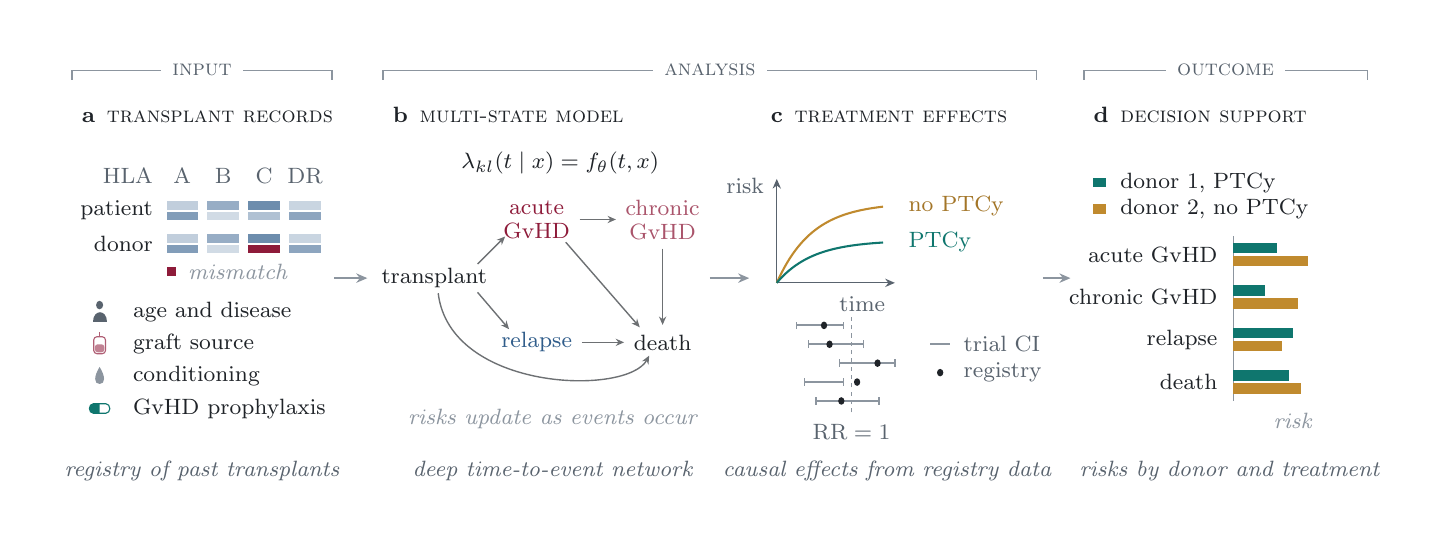
\begin{tikzpicture}[
    yscale=1.2,
    font=\footnotesize, text=ink,
    show background rectangle,
    background rectangle/.style={fill=white},
    inner frame sep=10pt,
    title/.style={anchor=base west, font=\footnotesize},
    sub/.style={anchor=base, text=mute, font=\footnotesize\itshape},
    tag/.style={anchor=north, text=faint, font=\footnotesize\itshape},
    axis/.style={draw=mute, line width=0.45pt, -{Stealth[length=3.5pt, width=3pt]}},
    flow/.style={draw=faint, line width=0.6pt, -{Stealth[length=4pt, width=3.4pt]}},
    group/.style={draw=faint, line width=0.5pt},
    grouplabel/.style={text=mute, font=\footnotesize\scshape, fill=white, inner xsep=4pt},
    move/.style={draw=ink!65, line width=0.5pt, -{Stealth[length=3pt, width=2.6pt]}}]

  % ---------------------------------------------------------- titles
  \node[title] at (-0.35,4.05) {\textbf{a}\enspace\textsc{transplant records}};
  \node[title] at (3.60,4.05)  {\textbf{b}\enspace\textsc{multi-state model}};
  \node[title] at (8.40,4.05)  {\textbf{c}\enspace\textsc{treatment effects}};
  \node[title] at (12.50,4.05) {\textbf{d}\enspace\textsc{decision support}};
  \draw[group] (-0.35,4.50) -- ++(0,0.10) -| (2.95,4.50);
  \node[grouplabel] at (1.30,4.60) {input};
  \draw[group] (3.60,4.50) -- ++(0,0.10) -| (11.90,4.50);
  \node[grouplabel] at (7.75,4.60) {analysis};
  \draw[group] (12.50,4.50) -- ++(0,0.10) -| (16.10,4.50);
  \node[grouplabel] at (14.30,4.60) {outcome};

  % ----------------------------------------------- a: transplant records
  % HLA typing at the four loci of an 8/8 match, two alleles each;
  % a matched donor allele repeats the patient's shade
  \node[anchor=base east, text=mute] at (0.80,3.40) {HLA};
  \foreach \l/\x in {A/1.05, B/1.57, C/2.09, DR/2.61}
    \node[anchor=base, text=mute] at (\x,3.40) {\l};
  \foreach \x/\a/\b in {1.05/30/60, 1.57/50/22, 2.09/70/38, 2.61/26/55} {
    \fill[slate!\a] (\x-0.20,3.125) rectangle (\x+0.20,3.215);
    \fill[slate!\b] (\x-0.20,3.015) rectangle (\x+0.20,3.105);
    \fill[slate!\a] (\x-0.20,2.775) rectangle (\x+0.20,2.865);
    \fill[slate!\b] (\x-0.20,2.665) rectangle (\x+0.20,2.755);
  }
  \fill[risk] (1.89,2.665) rectangle (2.29,2.755);                                 % C mismatch, 7/8
  \node[anchor=east] at (0.80,3.115) {patient};
  \node[anchor=east] at (0.80,2.765) {donor};
  \fill[risk] (0.85,2.42) rectangle ++(0.12,0.10);
  \node[anchor=west, text=faint, font=\footnotesize\itshape] at (1.00,2.47) {mismatch};

  \begin{scope}[shift={(0,2.04)}]                                   % age and disease
    \fill[mute] (0,0.075) circle (0.045);
    \fill[mute] (-0.09,-0.10) .. controls (-0.09,0.03) and (0.09,0.03) .. (0.09,-0.10) -- cycle;
  \end{scope}
  \begin{scope}[shift={(0,1.70)}]                                   % graft source
    \draw[risk!70, line width=0.4pt] (0,0.08) -- (0,0.13);
    \filldraw[fill=white, draw=risk!70, line width=0.4pt, rounded corners=1.2pt] (-0.075,-0.10) rectangle (0.075,0.08);
    \fill[risk!55, rounded corners=1pt] (-0.06,-0.085) rectangle (0.06,0.00);
  \end{scope}
  \begin{scope}[shift={(0,1.36)}]                                   % conditioning
    \fill[faint] (0,0.10) .. controls (0.075,0.00) and (0.075,-0.08) .. (0,-0.08)
      .. controls (-0.075,-0.08) and (-0.075,0.00) .. (0,0.10);
  \end{scope}
  \begin{scope}[shift={(0,1.02)}]                                   % GvHD prophylaxis
    \fill[ml] (0,-0.05) -- (-0.08,-0.05) arc[start angle=270, end angle=90, radius=0.05] -- (0,0.05) -- cycle;
    \draw[ml, line width=0.4pt] (-0.08,-0.05) -- (0.08,-0.05) arc[start angle=-90, end angle=90, radius=0.05]
      -- (-0.08,0.05) arc[start angle=90, end angle=270, radius=0.05] -- cycle;
  \end{scope}
  \foreach \y/\t in {2.04/age and disease, 1.70/graft source, 1.36/conditioning, 1.02/GvHD prophylaxis}
    \node[anchor=west] at (0.30,\y) {\t};

  % -------------------------------------------- b: multi-state model
  \node at (5.85,3.62) {$\lambda_{kl}(t \mid x) = f_\theta(t, x)$};
  \node (T) at (4.25,2.40) {transplant};
  \node[text=risk, align=center] (A) at (5.55,3.02) {acute\\[-1pt]GvHD};
  \node[text=risk!75, align=center] (C) at (7.15,3.02) {chronic\\[-1pt]GvHD};
  \node[text=slate] (R) at (5.55,1.72) {relapse};
  \node (D) at (7.15,1.72) {death};
  \draw[move] (4.80,2.55) -- (5.15,2.84);
  \draw[move] (4.80,2.25) -- (5.20,1.86);
  \draw[move] (A.east) -- (C.west);
  \draw[move] (C.south) -- (D.north);
  \draw[move] (R.east) -- (D.west);
  \draw[move] (5.92,2.78) -- (6.86,1.88);
  \draw[move] (4.30,2.24) .. controls (4.45,1.20) and (6.70,1.15) .. (6.98,1.58);
  \node[tag] at (5.75,1.12) {risks update as events occur};

  % --------------------------------------------- c: treatment effects
  \draw[axis] (8.60,2.35) -- (10.10,2.35);
  \draw[axis] (8.60,2.35) -- (8.60,3.45);
  \node[anchor=east, text=mute] at (8.56,3.38) {risk};
  \node[anchor=north east, text=mute] at (10.10,2.31) {time};
  \draw[ochre, line width=0.75pt] plot[domain=0:1.35, samples=60] ({8.60+\x},{2.35+0.85*(1-exp(-2.2*\x))});
  \draw[ml, line width=0.75pt] plot[domain=0:1.35, samples=60] ({8.60+\x},{2.35+0.45*(1-exp(-2.2*\x))});
  \node[anchor=west, text=ochre!85!black] at (10.15,3.16) {no PTCy};
  \node[anchor=west, text=ml] at (10.15,2.78) {PTCy};
  % registry estimates against the 95% intervals of randomized trials
  \draw[faint, line width=0.45pt, dash pattern=on 1.5pt off 1.5pt] (9.55,0.98) -- (9.55,2.02);
  \foreach \y/\lo/\e/\hi/\m in {1.90/8.85/9.15/9.45/9.20, 1.70/9.00/9.35/9.70/9.27, 1.50/9.40/9.75/10.10/9.88,
      1.30/8.95/9.20/9.45/9.62, 1.10/9.10/9.50/9.90/9.42} {
    \draw[faint, line width=0.7pt] (\lo,\y) -- (\hi,\y);
    \draw[faint, line width=0.5pt] (\lo,\y-0.04) -- ++(0,0.08) (\hi,\y-0.04) -- ++(0,0.08);
    \fill[ink] (\m,\y) circle (0.040);
  }
  \node[anchor=north, text=mute] at (9.55,0.96) {$\mathrm{RR} = 1$};
  \draw[faint, line width=0.7pt] (10.55,1.70) -- (10.80,1.70);
  \node[anchor=west, text=mute] at (10.85,1.70) {trial CI};
  \fill[ink] (10.675,1.40) circle (0.040);
  \node[anchor=west, text=mute] at (10.85,1.40) {registry};

  % ---------------------------------------------- d: decision support
  \fill[ml] (12.62,3.36) rectangle ++(0.16,0.10);
  \node[anchor=west] at (12.84,3.41) {donor 1, PTCy};
  \fill[ochre] (12.62,3.08) rectangle ++(0.16,0.10);
  \node[anchor=west] at (12.84,3.13) {donor 2, no PTCy};
  \draw[faint, line width=0.45pt] (14.40,1.10) -- (14.40,2.85);
  \foreach \y/\t/\a/\b in {2.65/acute GvHD/0.55/0.95, 2.20/chronic GvHD/0.40/0.82,
      1.75/relapse/0.75/0.62, 1.30/death/0.70/0.86} {
    \node[anchor=east] at (14.32,\y) {\t};
    \fill[ml] (14.40,\y+0.015) rectangle ++(\a,0.11);
    \fill[ochre] (14.40,\y-0.125) rectangle ++(\b,0.11);
  }
  \node[tag] at (15.15,1.08) {risk};

  % --------------------------------------------------- panel notes
  \node[sub] at (1.30,0.30)  {registry of past transplants};
  \node[sub] at (5.75,0.30)  {deep time-to-event network};
  \node[sub] at (10.00,0.30) {causal effects from registry data};
  \node[sub] at (14.35,0.30) {risks by donor and treatment};

  \draw[flow] (2.98,2.40) -- (3.40,2.40);
  \draw[flow] (7.75,2.40) -- (8.25,2.40);
  \draw[flow] (11.98,2.40) -- (12.33,2.40);
\end{tikzpicture}
\end{document}
"
%          dvisvgm --no-fonts --exact-bbox --optimize research_match.dvi
\documentclass[tikz,border=0pt]{standalone}
\usepackage[T1]{fontenc}
\usepackage{lmodern}
\usepackage{amsmath}
\usetikzlibrary{arrows.meta,backgrounds}

\definecolor{ink}{HTML}{1F2328}
\definecolor{mute}{HTML}{59636E}
\definecolor{faint}{HTML}{8C959F}
\definecolor{rule}{HTML}{D0D7DE}
\definecolor{risk}{HTML}{8E1B3A}
\definecolor{ochre}{HTML}{C08A2E}
\definecolor{slate}{HTML}{2F5C8A}
\definecolor{ml}{HTML}{0F766E}

\begin{document}
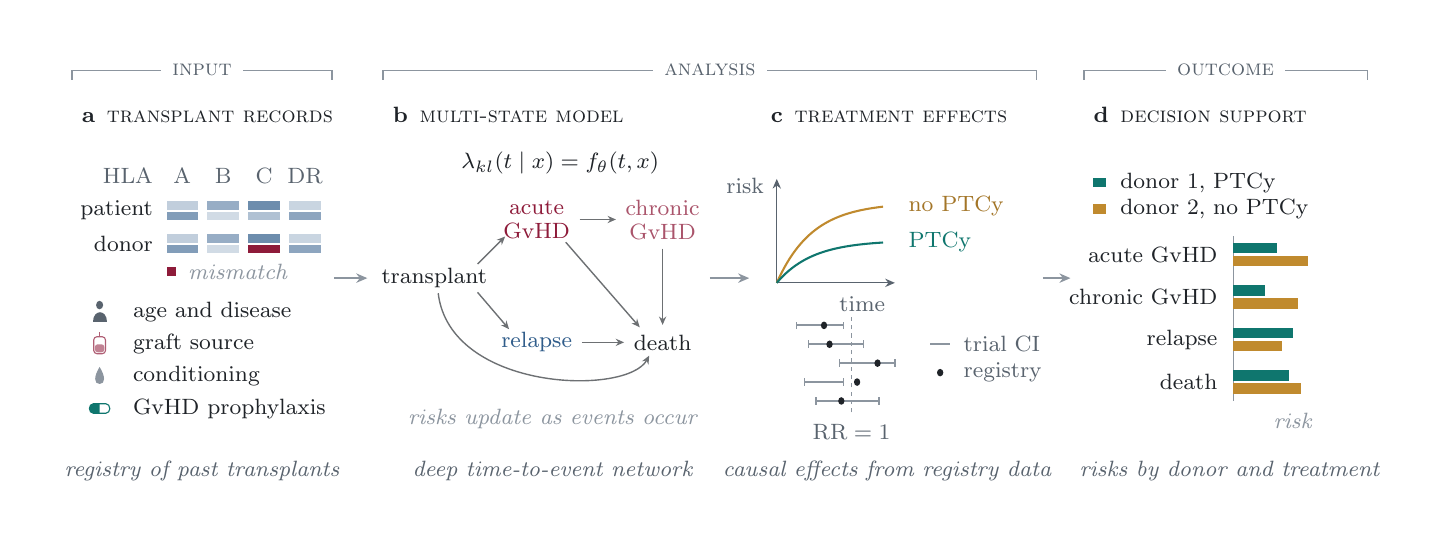
\begin{tikzpicture}[
    yscale=1.2,
    font=\footnotesize, text=ink,
    show background rectangle,
    background rectangle/.style={fill=white},
    inner frame sep=10pt,
    title/.style={anchor=base west, font=\footnotesize},
    sub/.style={anchor=base, text=mute, font=\footnotesize\itshape},
    tag/.style={anchor=north, text=faint, font=\footnotesize\itshape},
    axis/.style={draw=mute, line width=0.45pt, -{Stealth[length=3.5pt, width=3pt]}},
    flow/.style={draw=faint, line width=0.6pt, -{Stealth[length=4pt, width=3.4pt]}},
    group/.style={draw=faint, line width=0.5pt},
    grouplabel/.style={text=mute, font=\footnotesize\scshape, fill=white, inner xsep=4pt},
    move/.style={draw=ink!65, line width=0.5pt, -{Stealth[length=3pt, width=2.6pt]}}]

  % ---------------------------------------------------------- titles
  \node[title] at (-0.35,4.05) {\textbf{a}\enspace\textsc{transplant records}};
  \node[title] at (3.60,4.05)  {\textbf{b}\enspace\textsc{multi-state model}};
  \node[title] at (8.40,4.05)  {\textbf{c}\enspace\textsc{treatment effects}};
  \node[title] at (12.50,4.05) {\textbf{d}\enspace\textsc{decision support}};
  \draw[group] (-0.35,4.50) -- ++(0,0.10) -| (2.95,4.50);
  \node[grouplabel] at (1.30,4.60) {input};
  \draw[group] (3.60,4.50) -- ++(0,0.10) -| (11.90,4.50);
  \node[grouplabel] at (7.75,4.60) {analysis};
  \draw[group] (12.50,4.50) -- ++(0,0.10) -| (16.10,4.50);
  \node[grouplabel] at (14.30,4.60) {outcome};

  % ----------------------------------------------- a: transplant records
  % HLA typing at the four loci of an 8/8 match, two alleles each;
  % a matched donor allele repeats the patient's shade
  \node[anchor=base east, text=mute] at (0.80,3.40) {HLA};
  \foreach \l/\x in {A/1.05, B/1.57, C/2.09, DR/2.61}
    \node[anchor=base, text=mute] at (\x,3.40) {\l};
  \foreach \x/\a/\b in {1.05/30/60, 1.57/50/22, 2.09/70/38, 2.61/26/55} {
    \fill[slate!\a] (\x-0.20,3.125) rectangle (\x+0.20,3.215);
    \fill[slate!\b] (\x-0.20,3.015) rectangle (\x+0.20,3.105);
    \fill[slate!\a] (\x-0.20,2.775) rectangle (\x+0.20,2.865);
    \fill[slate!\b] (\x-0.20,2.665) rectangle (\x+0.20,2.755);
  }
  \fill[risk] (1.89,2.665) rectangle (2.29,2.755);                                 % C mismatch, 7/8
  \node[anchor=east] at (0.80,3.115) {patient};
  \node[anchor=east] at (0.80,2.765) {donor};
  \fill[risk] (0.85,2.42) rectangle ++(0.12,0.10);
  \node[anchor=west, text=faint, font=\footnotesize\itshape] at (1.00,2.47) {mismatch};

  \begin{scope}[shift={(0,2.04)}]                                   % age and disease
    \fill[mute] (0,0.075) circle (0.045);
    \fill[mute] (-0.09,-0.10) .. controls (-0.09,0.03) and (0.09,0.03) .. (0.09,-0.10) -- cycle;
  \end{scope}
  \begin{scope}[shift={(0,1.70)}]                                   % graft source
    \draw[risk!70, line width=0.4pt] (0,0.08) -- (0,0.13);
    \filldraw[fill=white, draw=risk!70, line width=0.4pt, rounded corners=1.2pt] (-0.075,-0.10) rectangle (0.075,0.08);
    \fill[risk!55, rounded corners=1pt] (-0.06,-0.085) rectangle (0.06,0.00);
  \end{scope}
  \begin{scope}[shift={(0,1.36)}]                                   % conditioning
    \fill[faint] (0,0.10) .. controls (0.075,0.00) and (0.075,-0.08) .. (0,-0.08)
      .. controls (-0.075,-0.08) and (-0.075,0.00) .. (0,0.10);
  \end{scope}
  \begin{scope}[shift={(0,1.02)}]                                   % GvHD prophylaxis
    \fill[ml] (0,-0.05) -- (-0.08,-0.05) arc[start angle=270, end angle=90, radius=0.05] -- (0,0.05) -- cycle;
    \draw[ml, line width=0.4pt] (-0.08,-0.05) -- (0.08,-0.05) arc[start angle=-90, end angle=90, radius=0.05]
      -- (-0.08,0.05) arc[start angle=90, end angle=270, radius=0.05] -- cycle;
  \end{scope}
  \foreach \y/\t in {2.04/age and disease, 1.70/graft source, 1.36/conditioning, 1.02/GvHD prophylaxis}
    \node[anchor=west] at (0.30,\y) {\t};

  % -------------------------------------------- b: multi-state model
  \node at (5.85,3.62) {$\lambda_{kl}(t \mid x) = f_\theta(t, x)$};
  \node (T) at (4.25,2.40) {transplant};
  \node[text=risk, align=center] (A) at (5.55,3.02) {acute\\[-1pt]GvHD};
  \node[text=risk!75, align=center] (C) at (7.15,3.02) {chronic\\[-1pt]GvHD};
  \node[text=slate] (R) at (5.55,1.72) {relapse};
  \node (D) at (7.15,1.72) {death};
  \draw[move] (4.80,2.55) -- (5.15,2.84);
  \draw[move] (4.80,2.25) -- (5.20,1.86);
  \draw[move] (A.east) -- (C.west);
  \draw[move] (C.south) -- (D.north);
  \draw[move] (R.east) -- (D.west);
  \draw[move] (5.92,2.78) -- (6.86,1.88);
  \draw[move] (4.30,2.24) .. controls (4.45,1.20) and (6.70,1.15) .. (6.98,1.58);
  \node[tag] at (5.75,1.12) {risks update as events occur};

  % --------------------------------------------- c: treatment effects
  \draw[axis] (8.60,2.35) -- (10.10,2.35);
  \draw[axis] (8.60,2.35) -- (8.60,3.45);
  \node[anchor=east, text=mute] at (8.56,3.38) {risk};
  \node[anchor=north east, text=mute] at (10.10,2.31) {time};
  \draw[ochre, line width=0.75pt] plot[domain=0:1.35, samples=60] ({8.60+\x},{2.35+0.85*(1-exp(-2.2*\x))});
  \draw[ml, line width=0.75pt] plot[domain=0:1.35, samples=60] ({8.60+\x},{2.35+0.45*(1-exp(-2.2*\x))});
  \node[anchor=west, text=ochre!85!black] at (10.15,3.16) {no PTCy};
  \node[anchor=west, text=ml] at (10.15,2.78) {PTCy};
  % registry estimates against the 95% intervals of randomized trials
  \draw[faint, line width=0.45pt, dash pattern=on 1.5pt off 1.5pt] (9.55,0.98) -- (9.55,2.02);
  \foreach \y/\lo/\e/\hi/\m in {1.90/8.85/9.15/9.45/9.20, 1.70/9.00/9.35/9.70/9.27, 1.50/9.40/9.75/10.10/9.88,
      1.30/8.95/9.20/9.45/9.62, 1.10/9.10/9.50/9.90/9.42} {
    \draw[faint, line width=0.7pt] (\lo,\y) -- (\hi,\y);
    \draw[faint, line width=0.5pt] (\lo,\y-0.04) -- ++(0,0.08) (\hi,\y-0.04) -- ++(0,0.08);
    \fill[ink] (\m,\y) circle (0.040);
  }
  \node[anchor=north, text=mute] at (9.55,0.96) {$\mathrm{RR} = 1$};
  \draw[faint, line width=0.7pt] (10.55,1.70) -- (10.80,1.70);
  \node[anchor=west, text=mute] at (10.85,1.70) {trial CI};
  \fill[ink] (10.675,1.40) circle (0.040);
  \node[anchor=west, text=mute] at (10.85,1.40) {registry};

  % ---------------------------------------------- d: decision support
  \fill[ml] (12.62,3.36) rectangle ++(0.16,0.10);
  \node[anchor=west] at (12.84,3.41) {donor 1, PTCy};
  \fill[ochre] (12.62,3.08) rectangle ++(0.16,0.10);
  \node[anchor=west] at (12.84,3.13) {donor 2, no PTCy};
  \draw[faint, line width=0.45pt] (14.40,1.10) -- (14.40,2.85);
  \foreach \y/\t/\a/\b in {2.65/acute GvHD/0.55/0.95, 2.20/chronic GvHD/0.40/0.82,
      1.75/relapse/0.75/0.62, 1.30/death/0.70/0.86} {
    \node[anchor=east] at (14.32,\y) {\t};
    \fill[ml] (14.40,\y+0.015) rectangle ++(\a,0.11);
    \fill[ochre] (14.40,\y-0.125) rectangle ++(\b,0.11);
  }
  \node[tag] at (15.15,1.08) {risk};

  % --------------------------------------------------- panel notes
  \node[sub] at (1.30,0.30)  {registry of past transplants};
  \node[sub] at (5.75,0.30)  {deep time-to-event network};
  \node[sub] at (10.00,0.30) {causal effects from registry data};
  \node[sub] at (14.35,0.30) {risks by donor and treatment};

  \draw[flow] (2.98,2.40) -- (3.40,2.40);
  \draw[flow] (7.75,2.40) -- (8.25,2.40);
  \draw[flow] (11.98,2.40) -- (12.33,2.40);
\end{tikzpicture}
\end{document}
"
%          dvisvgm --no-fonts --exact-bbox --optimize research_match.dvi
\documentclass[tikz,border=0pt]{standalone}
\usepackage[T1]{fontenc}
\usepackage{lmodern}
\usepackage{amsmath}
\usetikzlibrary{arrows.meta,backgrounds}

\definecolor{ink}{HTML}{1F2328}
\definecolor{mute}{HTML}{59636E}
\definecolor{faint}{HTML}{8C959F}
\definecolor{rule}{HTML}{D0D7DE}
\definecolor{risk}{HTML}{8E1B3A}
\definecolor{ochre}{HTML}{C08A2E}
\definecolor{slate}{HTML}{2F5C8A}
\definecolor{ml}{HTML}{0F766E}

\begin{document}
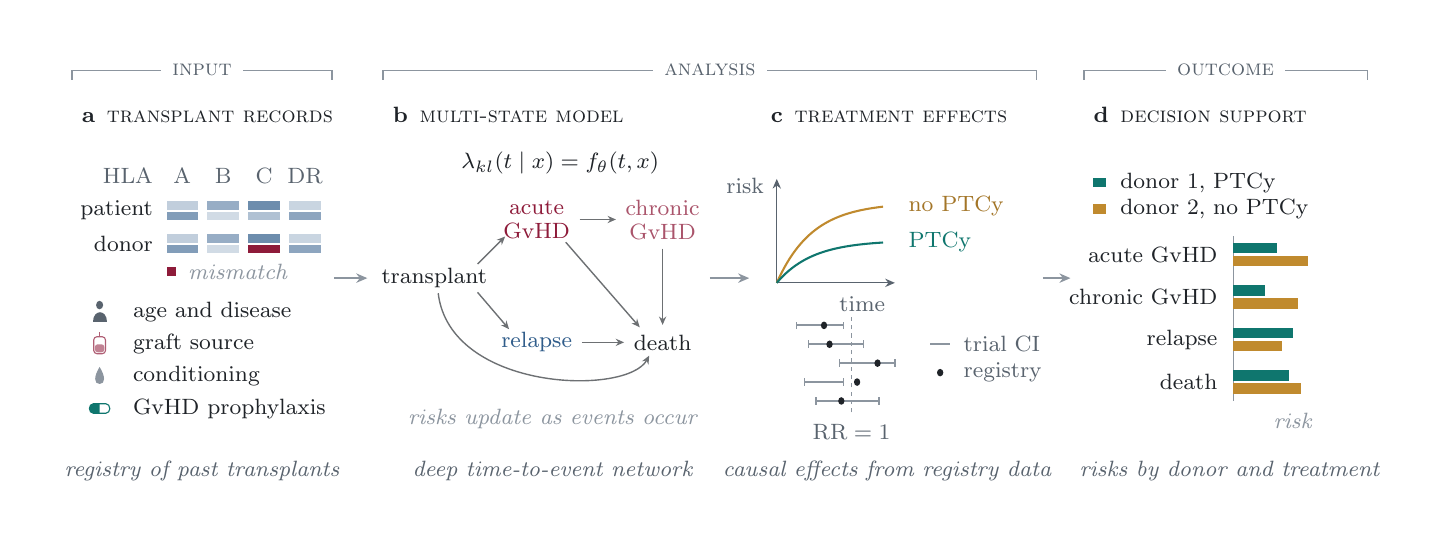
\begin{tikzpicture}[
    yscale=1.2,
    font=\footnotesize, text=ink,
    show background rectangle,
    background rectangle/.style={fill=white},
    inner frame sep=10pt,
    title/.style={anchor=base west, font=\footnotesize},
    sub/.style={anchor=base, text=mute, font=\footnotesize\itshape},
    tag/.style={anchor=north, text=faint, font=\footnotesize\itshape},
    axis/.style={draw=mute, line width=0.45pt, -{Stealth[length=3.5pt, width=3pt]}},
    flow/.style={draw=faint, line width=0.6pt, -{Stealth[length=4pt, width=3.4pt]}},
    group/.style={draw=faint, line width=0.5pt},
    grouplabel/.style={text=mute, font=\footnotesize\scshape, fill=white, inner xsep=4pt},
    move/.style={draw=ink!65, line width=0.5pt, -{Stealth[length=3pt, width=2.6pt]}}]

  % ---------------------------------------------------------- titles
  \node[title] at (-0.35,4.05) {\textbf{a}\enspace\textsc{transplant records}};
  \node[title] at (3.60,4.05)  {\textbf{b}\enspace\textsc{multi-state model}};
  \node[title] at (8.40,4.05)  {\textbf{c}\enspace\textsc{treatment effects}};
  \node[title] at (12.50,4.05) {\textbf{d}\enspace\textsc{decision support}};
  \draw[group] (-0.35,4.50) -- ++(0,0.10) -| (2.95,4.50);
  \node[grouplabel] at (1.30,4.60) {input};
  \draw[group] (3.60,4.50) -- ++(0,0.10) -| (11.90,4.50);
  \node[grouplabel] at (7.75,4.60) {analysis};
  \draw[group] (12.50,4.50) -- ++(0,0.10) -| (16.10,4.50);
  \node[grouplabel] at (14.30,4.60) {outcome};

  % ----------------------------------------------- a: transplant records
  % HLA typing at the four loci of an 8/8 match, two alleles each;
  % a matched donor allele repeats the patient's shade
  \node[anchor=base east, text=mute] at (0.80,3.40) {HLA};
  \foreach \l/\x in {A/1.05, B/1.57, C/2.09, DR/2.61}
    \node[anchor=base, text=mute] at (\x,3.40) {\l};
  \foreach \x/\a/\b in {1.05/30/60, 1.57/50/22, 2.09/70/38, 2.61/26/55} {
    \fill[slate!\a] (\x-0.20,3.125) rectangle (\x+0.20,3.215);
    \fill[slate!\b] (\x-0.20,3.015) rectangle (\x+0.20,3.105);
    \fill[slate!\a] (\x-0.20,2.775) rectangle (\x+0.20,2.865);
    \fill[slate!\b] (\x-0.20,2.665) rectangle (\x+0.20,2.755);
  }
  \fill[risk] (1.89,2.665) rectangle (2.29,2.755);                                 % C mismatch, 7/8
  \node[anchor=east] at (0.80,3.115) {patient};
  \node[anchor=east] at (0.80,2.765) {donor};
  \fill[risk] (0.85,2.42) rectangle ++(0.12,0.10);
  \node[anchor=west, text=faint, font=\footnotesize\itshape] at (1.00,2.47) {mismatch};

  \begin{scope}[shift={(0,2.04)}]                                   % age and disease
    \fill[mute] (0,0.075) circle (0.045);
    \fill[mute] (-0.09,-0.10) .. controls (-0.09,0.03) and (0.09,0.03) .. (0.09,-0.10) -- cycle;
  \end{scope}
  \begin{scope}[shift={(0,1.70)}]                                   % graft source
    \draw[risk!70, line width=0.4pt] (0,0.08) -- (0,0.13);
    \filldraw[fill=white, draw=risk!70, line width=0.4pt, rounded corners=1.2pt] (-0.075,-0.10) rectangle (0.075,0.08);
    \fill[risk!55, rounded corners=1pt] (-0.06,-0.085) rectangle (0.06,0.00);
  \end{scope}
  \begin{scope}[shift={(0,1.36)}]                                   % conditioning
    \fill[faint] (0,0.10) .. controls (0.075,0.00) and (0.075,-0.08) .. (0,-0.08)
      .. controls (-0.075,-0.08) and (-0.075,0.00) .. (0,0.10);
  \end{scope}
  \begin{scope}[shift={(0,1.02)}]                                   % GvHD prophylaxis
    \fill[ml] (0,-0.05) -- (-0.08,-0.05) arc[start angle=270, end angle=90, radius=0.05] -- (0,0.05) -- cycle;
    \draw[ml, line width=0.4pt] (-0.08,-0.05) -- (0.08,-0.05) arc[start angle=-90, end angle=90, radius=0.05]
      -- (-0.08,0.05) arc[start angle=90, end angle=270, radius=0.05] -- cycle;
  \end{scope}
  \foreach \y/\t in {2.04/age and disease, 1.70/graft source, 1.36/conditioning, 1.02/GvHD prophylaxis}
    \node[anchor=west] at (0.30,\y) {\t};

  % -------------------------------------------- b: multi-state model
  \node at (5.85,3.62) {$\lambda_{kl}(t \mid x) = f_\theta(t, x)$};
  \node (T) at (4.25,2.40) {transplant};
  \node[text=risk, align=center] (A) at (5.55,3.02) {acute\\[-1pt]GvHD};
  \node[text=risk!75, align=center] (C) at (7.15,3.02) {chronic\\[-1pt]GvHD};
  \node[text=slate] (R) at (5.55,1.72) {relapse};
  \node (D) at (7.15,1.72) {death};
  \draw[move] (4.80,2.55) -- (5.15,2.84);
  \draw[move] (4.80,2.25) -- (5.20,1.86);
  \draw[move] (A.east) -- (C.west);
  \draw[move] (C.south) -- (D.north);
  \draw[move] (R.east) -- (D.west);
  \draw[move] (5.92,2.78) -- (6.86,1.88);
  \draw[move] (4.30,2.24) .. controls (4.45,1.20) and (6.70,1.15) .. (6.98,1.58);
  \node[tag] at (5.75,1.12) {risks update as events occur};

  % --------------------------------------------- c: treatment effects
  \draw[axis] (8.60,2.35) -- (10.10,2.35);
  \draw[axis] (8.60,2.35) -- (8.60,3.45);
  \node[anchor=east, text=mute] at (8.56,3.38) {risk};
  \node[anchor=north east, text=mute] at (10.10,2.31) {time};
  \draw[ochre, line width=0.75pt] plot[domain=0:1.35, samples=60] ({8.60+\x},{2.35+0.85*(1-exp(-2.2*\x))});
  \draw[ml, line width=0.75pt] plot[domain=0:1.35, samples=60] ({8.60+\x},{2.35+0.45*(1-exp(-2.2*\x))});
  \node[anchor=west, text=ochre!85!black] at (10.15,3.16) {no PTCy};
  \node[anchor=west, text=ml] at (10.15,2.78) {PTCy};
  % registry estimates against the 95% intervals of randomized trials
  \draw[faint, line width=0.45pt, dash pattern=on 1.5pt off 1.5pt] (9.55,0.98) -- (9.55,2.02);
  \foreach \y/\lo/\e/\hi/\m in {1.90/8.85/9.15/9.45/9.20, 1.70/9.00/9.35/9.70/9.27, 1.50/9.40/9.75/10.10/9.88,
      1.30/8.95/9.20/9.45/9.62, 1.10/9.10/9.50/9.90/9.42} {
    \draw[faint, line width=0.7pt] (\lo,\y) -- (\hi,\y);
    \draw[faint, line width=0.5pt] (\lo,\y-0.04) -- ++(0,0.08) (\hi,\y-0.04) -- ++(0,0.08);
    \fill[ink] (\m,\y) circle (0.040);
  }
  \node[anchor=north, text=mute] at (9.55,0.96) {$\mathrm{RR} = 1$};
  \draw[faint, line width=0.7pt] (10.55,1.70) -- (10.80,1.70);
  \node[anchor=west, text=mute] at (10.85,1.70) {trial CI};
  \fill[ink] (10.675,1.40) circle (0.040);
  \node[anchor=west, text=mute] at (10.85,1.40) {registry};

  % ---------------------------------------------- d: decision support
  \fill[ml] (12.62,3.36) rectangle ++(0.16,0.10);
  \node[anchor=west] at (12.84,3.41) {donor 1, PTCy};
  \fill[ochre] (12.62,3.08) rectangle ++(0.16,0.10);
  \node[anchor=west] at (12.84,3.13) {donor 2, no PTCy};
  \draw[faint, line width=0.45pt] (14.40,1.10) -- (14.40,2.85);
  \foreach \y/\t/\a/\b in {2.65/acute GvHD/0.55/0.95, 2.20/chronic GvHD/0.40/0.82,
      1.75/relapse/0.75/0.62, 1.30/death/0.70/0.86} {
    \node[anchor=east] at (14.32,\y) {\t};
    \fill[ml] (14.40,\y+0.015) rectangle ++(\a,0.11);
    \fill[ochre] (14.40,\y-0.125) rectangle ++(\b,0.11);
  }
  \node[tag] at (15.15,1.08) {risk};

  % --------------------------------------------------- panel notes
  \node[sub] at (1.30,0.30)  {registry of past transplants};
  \node[sub] at (5.75,0.30)  {deep time-to-event network};
  \node[sub] at (10.00,0.30) {causal effects from registry data};
  \node[sub] at (14.35,0.30) {risks by donor and treatment};

  \draw[flow] (2.98,2.40) -- (3.40,2.40);
  \draw[flow] (7.75,2.40) -- (8.25,2.40);
  \draw[flow] (11.98,2.40) -- (12.33,2.40);
\end{tikzpicture}
\end{document}
"
%          dvisvgm --no-fonts --exact-bbox --optimize research_match.dvi
\documentclass[tikz,border=0pt]{standalone}
\usepackage[T1]{fontenc}
\usepackage{lmodern}
\usepackage{amsmath}
\usetikzlibrary{arrows.meta,backgrounds}

\definecolor{ink}{HTML}{1F2328}
\definecolor{mute}{HTML}{59636E}
\definecolor{faint}{HTML}{8C959F}
\definecolor{rule}{HTML}{D0D7DE}
\definecolor{risk}{HTML}{8E1B3A}
\definecolor{ochre}{HTML}{C08A2E}
\definecolor{slate}{HTML}{2F5C8A}
\definecolor{ml}{HTML}{0F766E}

\begin{document}
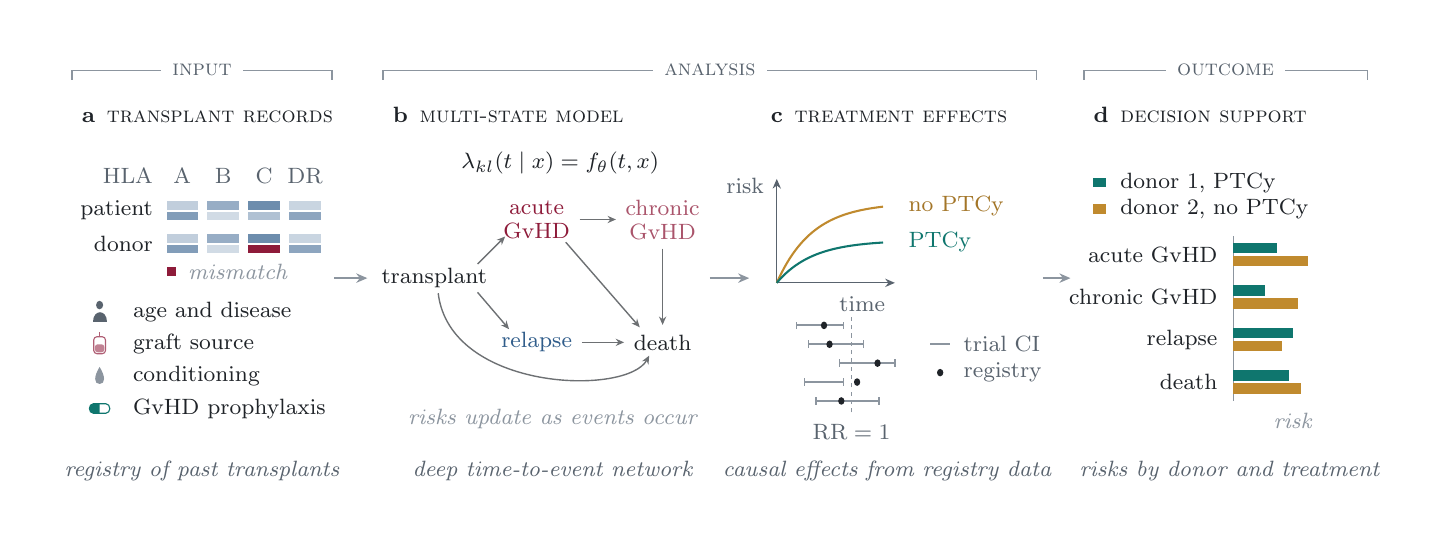
\begin{tikzpicture}[
    yscale=1.2,
    font=\footnotesize, text=ink,
    show background rectangle,
    background rectangle/.style={fill=white},
    inner frame sep=10pt,
    title/.style={anchor=base west, font=\footnotesize},
    sub/.style={anchor=base, text=mute, font=\footnotesize\itshape},
    tag/.style={anchor=north, text=faint, font=\footnotesize\itshape},
    axis/.style={draw=mute, line width=0.45pt, -{Stealth[length=3.5pt, width=3pt]}},
    flow/.style={draw=faint, line width=0.6pt, -{Stealth[length=4pt, width=3.4pt]}},
    group/.style={draw=faint, line width=0.5pt},
    grouplabel/.style={text=mute, font=\footnotesize\scshape, fill=white, inner xsep=4pt},
    move/.style={draw=ink!65, line width=0.5pt, -{Stealth[length=3pt, width=2.6pt]}}]

  % ---------------------------------------------------------- titles
  \node[title] at (-0.35,4.05) {\textbf{a}\enspace\textsc{transplant records}};
  \node[title] at (3.60,4.05)  {\textbf{b}\enspace\textsc{multi-state model}};
  \node[title] at (8.40,4.05)  {\textbf{c}\enspace\textsc{treatment effects}};
  \node[title] at (12.50,4.05) {\textbf{d}\enspace\textsc{decision support}};
  \draw[group] (-0.35,4.50) -- ++(0,0.10) -| (2.95,4.50);
  \node[grouplabel] at (1.30,4.60) {input};
  \draw[group] (3.60,4.50) -- ++(0,0.10) -| (11.90,4.50);
  \node[grouplabel] at (7.75,4.60) {analysis};
  \draw[group] (12.50,4.50) -- ++(0,0.10) -| (16.10,4.50);
  \node[grouplabel] at (14.30,4.60) {outcome};

  % ----------------------------------------------- a: transplant records
  % HLA typing at the four loci of an 8/8 match, two alleles each;
  % a matched donor allele repeats the patient's shade
  \node[anchor=base east, text=mute] at (0.80,3.40) {HLA};
  \foreach \l/\x in {A/1.05, B/1.57, C/2.09, DR/2.61}
    \node[anchor=base, text=mute] at (\x,3.40) {\l};
  \foreach \x/\a/\b in {1.05/30/60, 1.57/50/22, 2.09/70/38, 2.61/26/55} {
    \fill[slate!\a] (\x-0.20,3.125) rectangle (\x+0.20,3.215);
    \fill[slate!\b] (\x-0.20,3.015) rectangle (\x+0.20,3.105);
    \fill[slate!\a] (\x-0.20,2.775) rectangle (\x+0.20,2.865);
    \fill[slate!\b] (\x-0.20,2.665) rectangle (\x+0.20,2.755);
  }
  \fill[risk] (1.89,2.665) rectangle (2.29,2.755);                                 % C mismatch, 7/8
  \node[anchor=east] at (0.80,3.115) {patient};
  \node[anchor=east] at (0.80,2.765) {donor};
  \fill[risk] (0.85,2.42) rectangle ++(0.12,0.10);
  \node[anchor=west, text=faint, font=\footnotesize\itshape] at (1.00,2.47) {mismatch};

  \begin{scope}[shift={(0,2.04)}]                                   % age and disease
    \fill[mute] (0,0.075) circle (0.045);
    \fill[mute] (-0.09,-0.10) .. controls (-0.09,0.03) and (0.09,0.03) .. (0.09,-0.10) -- cycle;
  \end{scope}
  \begin{scope}[shift={(0,1.70)}]                                   % graft source
    \draw[risk!70, line width=0.4pt] (0,0.08) -- (0,0.13);
    \filldraw[fill=white, draw=risk!70, line width=0.4pt, rounded corners=1.2pt] (-0.075,-0.10) rectangle (0.075,0.08);
    \fill[risk!55, rounded corners=1pt] (-0.06,-0.085) rectangle (0.06,0.00);
  \end{scope}
  \begin{scope}[shift={(0,1.36)}]                                   % conditioning
    \fill[faint] (0,0.10) .. controls (0.075,0.00) and (0.075,-0.08) .. (0,-0.08)
      .. controls (-0.075,-0.08) and (-0.075,0.00) .. (0,0.10);
  \end{scope}
  \begin{scope}[shift={(0,1.02)}]                                   % GvHD prophylaxis
    \fill[ml] (0,-0.05) -- (-0.08,-0.05) arc[start angle=270, end angle=90, radius=0.05] -- (0,0.05) -- cycle;
    \draw[ml, line width=0.4pt] (-0.08,-0.05) -- (0.08,-0.05) arc[start angle=-90, end angle=90, radius=0.05]
      -- (-0.08,0.05) arc[start angle=90, end angle=270, radius=0.05] -- cycle;
  \end{scope}
  \foreach \y/\t in {2.04/age and disease, 1.70/graft source, 1.36/conditioning, 1.02/GvHD prophylaxis}
    \node[anchor=west] at (0.30,\y) {\t};

  % -------------------------------------------- b: multi-state model
  \node at (5.85,3.62) {$\lambda_{kl}(t \mid x) = f_\theta(t, x)$};
  \node (T) at (4.25,2.40) {transplant};
  \node[text=risk, align=center] (A) at (5.55,3.02) {acute\\[-1pt]GvHD};
  \node[text=risk!75, align=center] (C) at (7.15,3.02) {chronic\\[-1pt]GvHD};
  \node[text=slate] (R) at (5.55,1.72) {relapse};
  \node (D) at (7.15,1.72) {death};
  \draw[move] (4.80,2.55) -- (5.15,2.84);
  \draw[move] (4.80,2.25) -- (5.20,1.86);
  \draw[move] (A.east) -- (C.west);
  \draw[move] (C.south) -- (D.north);
  \draw[move] (R.east) -- (D.west);
  \draw[move] (5.92,2.78) -- (6.86,1.88);
  \draw[move] (4.30,2.24) .. controls (4.45,1.20) and (6.70,1.15) .. (6.98,1.58);
  \node[tag] at (5.75,1.12) {risks update as events occur};

  % --------------------------------------------- c: treatment effects
  \draw[axis] (8.60,2.35) -- (10.10,2.35);
  \draw[axis] (8.60,2.35) -- (8.60,3.45);
  \node[anchor=east, text=mute] at (8.56,3.38) {risk};
  \node[anchor=north east, text=mute] at (10.10,2.31) {time};
  \draw[ochre, line width=0.75pt] plot[domain=0:1.35, samples=60] ({8.60+\x},{2.35+0.85*(1-exp(-2.2*\x))});
  \draw[ml, line width=0.75pt] plot[domain=0:1.35, samples=60] ({8.60+\x},{2.35+0.45*(1-exp(-2.2*\x))});
  \node[anchor=west, text=ochre!85!black] at (10.15,3.16) {no PTCy};
  \node[anchor=west, text=ml] at (10.15,2.78) {PTCy};
  % registry estimates against the 95% intervals of randomized trials
  \draw[faint, line width=0.45pt, dash pattern=on 1.5pt off 1.5pt] (9.55,0.98) -- (9.55,2.02);
  \foreach \y/\lo/\e/\hi/\m in {1.90/8.85/9.15/9.45/9.20, 1.70/9.00/9.35/9.70/9.27, 1.50/9.40/9.75/10.10/9.88,
      1.30/8.95/9.20/9.45/9.62, 1.10/9.10/9.50/9.90/9.42} {
    \draw[faint, line width=0.7pt] (\lo,\y) -- (\hi,\y);
    \draw[faint, line width=0.5pt] (\lo,\y-0.04) -- ++(0,0.08) (\hi,\y-0.04) -- ++(0,0.08);
    \fill[ink] (\m,\y) circle (0.040);
  }
  \node[anchor=north, text=mute] at (9.55,0.96) {$\mathrm{RR} = 1$};
  \draw[faint, line width=0.7pt] (10.55,1.70) -- (10.80,1.70);
  \node[anchor=west, text=mute] at (10.85,1.70) {trial CI};
  \fill[ink] (10.675,1.40) circle (0.040);
  \node[anchor=west, text=mute] at (10.85,1.40) {registry};

  % ---------------------------------------------- d: decision support
  \fill[ml] (12.62,3.36) rectangle ++(0.16,0.10);
  \node[anchor=west] at (12.84,3.41) {donor 1, PTCy};
  \fill[ochre] (12.62,3.08) rectangle ++(0.16,0.10);
  \node[anchor=west] at (12.84,3.13) {donor 2, no PTCy};
  \draw[faint, line width=0.45pt] (14.40,1.10) -- (14.40,2.85);
  \foreach \y/\t/\a/\b in {2.65/acute GvHD/0.55/0.95, 2.20/chronic GvHD/0.40/0.82,
      1.75/relapse/0.75/0.62, 1.30/death/0.70/0.86} {
    \node[anchor=east] at (14.32,\y) {\t};
    \fill[ml] (14.40,\y+0.015) rectangle ++(\a,0.11);
    \fill[ochre] (14.40,\y-0.125) rectangle ++(\b,0.11);
  }
  \node[tag] at (15.15,1.08) {risk};

  % --------------------------------------------------- panel notes
  \node[sub] at (1.30,0.30)  {registry of past transplants};
  \node[sub] at (5.75,0.30)  {deep time-to-event network};
  \node[sub] at (10.00,0.30) {causal effects from registry data};
  \node[sub] at (14.35,0.30) {risks by donor and treatment};

  \draw[flow] (2.98,2.40) -- (3.40,2.40);
  \draw[flow] (7.75,2.40) -- (8.25,2.40);
  \draw[flow] (11.98,2.40) -- (12.33,2.40);
\end{tikzpicture}
\end{document}
